% Drawing 74/05-15 -- folder 74, batch 05, archive page 89 (PDF page 90).
% Transcription: Le diagramme. On y lit, sans pouvoir assurer le sens de toutes les flèches : en haut, $\mathrm{Car}_{d*}\simeq\mathrm{pav\,car}$, relié par des flèches marquées $2$ à $\mathrm{car}$, $\mathrm{car}_{\Omega}$ et $\mathrm{car}_{s*}$ ; au centre $S$, où aboutissent des flèches venant de $\mathrm{Ar}\xleftarrow{3}\mathrm{Arc}$ ($\simeq_3$ \uncertain{trig pt}, $\simeq_2$ trig ép), de « dodéc ép $\simeq$ pent ép $\simeq$ cour ép » et d'un schéma de « pent. » ; puis $\mathrm{hex}_{\mathrm{tr}*}$ ($\simeq$ pav pt $+$ tria), $\mathrm{hex}_{s*}\simeq\mathrm{car}_{r}$ ($\simeq$ pav $+$ tria $+$ \ill{}), $\mathrm{hex}_{\Omega^*}$ ($\mathfrak{S}_3$), $\mathrm{hex}_{\Omega}$ ($\mathfrak{S}_3$), $\mathrm{hex\,ép}\simeq\mathrm{car\,ép}$ ($G_{\mathrm{pav}}$ ; $\simeq$ pav ép, $\simeq$ car ép), $\mathrm{hex\,ép}'$ ($\mathfrak{S}_3$), $\mathrm{hex}_{d}$ ($\mathfrak{S}_2$ ; $\simeq$ tria pt $\simeq\mathrm{car}_{d}$) ; en bas, $\mathrm{Hex}$ ($\simeq$ tria \ill{}) $\xleftarrow[\mathrm{orr}]{2}\mathrm{Hex}_{s}\simeq\mathrm{hex}$ ($\simeq$ tria), $\mathrm{Hex}$ ($\simeq$ pav) $\xleftarrow[\mathrm{orr}]{2}$ ($\mathbb{D}_3$) $\mathrm{Hex}_{\mathrm{tr}}$ ($\simeq$ tr tria), ($\mathbb{D}_3$) $\mathrm{Hex\,ép}'$, ($\mathbb{D}_6$) $\mathrm{Hex\,ép}\simeq\mathrm{hex}_{\mathrm{tr}}$ ($\simeq$ tr ép tria ; $\mathfrak{S}_3$) $\xleftarrow{3}\mathrm{hex}_{s}\simeq\mathrm{car}_{s}$ ($\simeq$ tria ép ; $\mathfrak{S}_3$), $\mathrm{Hex}_{s*}$ ($\simeq$ ba pt), $\mathrm{Hex}_{\Omega}$, $\mathrm{Hex}_{t*}$ ($\simeq$ tri b tr), $\mathrm{Hex}_{tt*}$ ($\simeq$ tr $\circ$ tria ; $\mathbb{F}_2\times\mathbb{F}_2$), et la dernière ligne $\mathrm{triHex}$ ($\simeq$ tri pav) $\xleftarrow{3}\mathrm{pav}$, avec $\mathrm{Hex}\xrightarrow{3}\mathrm{triHex}$. Une bulle « échanges~! » renvoie par deux arcs de $\mathrm{hex\,ép}$ à lui-même. À gauche, une flèche « $\mathrm{b}\simeq$ doublet » et « bi pt ». À droite, des esquisses : trois prismes accolés, un pentagone subdivisé, une chaîne de points fléchés.
% Kind: large arrow diagram of sets of hexagons, squares and tilings, with sketches. Method 2 (schematic redraw from the facsimile). Status: partial.
% Notes: Landscape sheet. Nodes are placed where they stand, with their labels as the transcription reads them (illegible parts left out); the principal arrows are drawn with their degrees, many minor and doubled strokes are not, and the direction of some arrows is not certain (the transcription says so too). The « échanges ! » bubble returns by two arcs to hex ép. The sketches (pentagon schema at the upper left, three prisms, a subdivided pentagon, a chain of arrowed points at the right) are drawn as outlines. The texts at the upper right are not part of the figure.
% Coordinates: 1 unit = 1 mm = 1/100 of the crop width (bbox in page fractions: [0.08, 0.07, 0.98, 0.51]).
% Redrawn by Claude (claude-opus-5-5), issue #73, 2026-11-07; not checked by a human; not compiled (no TeX in the session).
% Rights: reproduces part of the work -- behind RENDER_TRANSCRIPTS, never published by itself.
\documentclass[tikz,border=3pt]{standalone}
\usepackage{amsmath,amssymb}
\usetikzlibrary{patterns,arrows.meta}
\tikzset{pencil/.style={black!45}, struck/.style={black!35}, mark/.style={circle,draw,inner sep=1.3pt}, pt/.style={circle,fill,inner sep=0.9pt}, opt/.style={circle,draw,fill=white,inner sep=1.1pt}}
\begin{document}
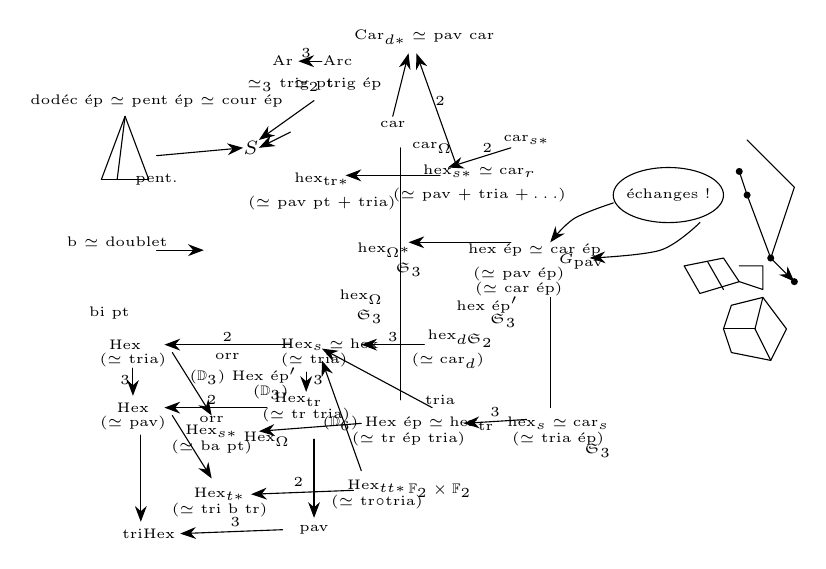
\begin{tikzpicture}[x=1mm,y=1mm,line cap=round,line join=round,font=\scriptsize]
\node[inner sep=1pt] at (44,-7) {\tiny $\mathrm{Car}_{d*}\simeq$ pav car};
\node[inner sep=1pt] at (40,-18) {\tiny car};
\node[inner sep=1pt] at (45,-21) {\tiny $\mathrm{car}_\Omega$};
\node[inner sep=1pt] at (57,-20) {\tiny $\mathrm{car}_{s*}$};
\node[inner sep=1pt] at (22,-21) {\scriptsize $S$};
\node[inner sep=1pt] at (26,-10) {\tiny Ar};
\draw[-{Stealth[length=2mm]}] (31,-10) -- (28,-10);
\node[inner sep=1pt] at (33,-10) {\tiny Arc};
\node[inner sep=1pt] at (29,-9) {\tiny $3$};
\node[inner sep=1pt] at (27,-13) {\tiny $\simeq_3$ trig pt};
\node[inner sep=1pt] at (33,-13) {\tiny $\simeq_2$ trig ép};
\node[inner sep=1pt] at (10,-15) {\tiny dodéc ép $\simeq$ pent ép $\simeq$ cour ép};
\draw (3,-25) -- (6,-17) -- (9,-25);
\draw (3,-25) -- (9,-25);
\draw (6,-17) -- (5,-25);
\node[inner sep=1pt] at (10,-25) {\tiny pent.};
\draw[-{Stealth[length=2mm]}] (10,-22) -- (21,-21);
\draw[-{Stealth[length=2mm]}] (27,-19) -- (23,-21);
\draw[-{Stealth[length=2mm]}] (30,-15) -- (23,-20);
\node[inner sep=1pt] at (31,-25) {\tiny $\mathrm{hex}_{\mathrm{tr}*}$};
\node[inner sep=1pt] at (31,-28) {\tiny ($\simeq$ pav pt $+$ tria)};
\node[inner sep=1pt] at (51,-24) {\tiny $\mathrm{hex}_{s*}\simeq\mathrm{car}_r$};
\node[inner sep=1pt] at (51,-27) {\tiny ($\simeq$ pav $+$ tria $+\ldots$)};
\node[inner sep=1pt] at (39,-34) {\tiny $\mathrm{hex}_{\Omega^*}$};
\node[inner sep=1pt] at (42,-36.5) {\tiny $\mathfrak S_3$};
\node[inner sep=1pt] at (36,-40) {\tiny $\mathrm{hex}_\Omega$};
\node[inner sep=1pt] at (37,-42.5) {\tiny $\mathfrak S_3$};
\node[inner sep=1pt] at (58,-34) {\tiny hex ép $\simeq$ car ép};
\node[inner sep=1pt] at (64,-35.5) {\tiny $G_{\mathrm{pav}}$};
\node[inner sep=1pt] at (56,-37) {\tiny ($\simeq$ pav ép)};
\node[inner sep=1pt] at (56,-39) {\tiny ($\simeq$ car ép)};
\node[inner sep=1pt] at (52,-41) {\tiny hex ép$'$};
\node[inner sep=1pt] at (54,-43) {\tiny $\mathfrak S_3$};
\node[inner sep=1pt] at (47,-45) {\tiny $\mathrm{hex}_d$};
\node[inner sep=1pt] at (51,-45.5) {\tiny $\mathfrak S_2$};
\node[inner sep=1pt] at (47,-48) {\tiny ($\simeq\mathrm{car}_d$)};
\node[inner sep=1pt] at (32,-46) {\tiny $\mathrm{Hex}_s\simeq\mathrm{hex}$};
\node[inner sep=1pt] at (30,-48) {\tiny ($\simeq$ tria)};
\node[inner sep=1pt] at (6,-46) {\tiny Hex};
\node[inner sep=1pt] at (7,-48) {\tiny ($\simeq$ tria)};
\node[inner sep=1pt] at (7,-54) {\tiny Hex};
\node[inner sep=1pt] at (7,-56) {\tiny ($\simeq$ pav)};
\node[inner sep=1pt] at (28,-53) {\tiny $\mathrm{Hex}_{\mathrm{tr}}$};
\node[inner sep=1pt] at (29,-55) {\tiny ($\simeq$ tr tria)};
\node[inner sep=1pt] at (24.5,-52) {\tiny ($\mathbb D_3$)};
\node[inner sep=1pt] at (21,-50) {\tiny ($\mathbb D_3$) Hex ép$'$};
\node[inner sep=1pt] at (46,-53) {\tiny tria};
\node[inner sep=1pt] at (42,-56) {\tiny ($\mathbb D_6$) Hex ép $\simeq\mathrm{hex}_{\mathrm{tr}}$};
\node[inner sep=1pt] at (42,-58) {\tiny ($\simeq$ tr ép tria)};
\node[inner sep=1pt] at (61,-56) {\tiny $\mathrm{hex}_s\simeq\mathrm{car}_s$};
\node[inner sep=1pt] at (61,-58) {\tiny ($\simeq$ tria ép)};
\node[inner sep=1pt] at (66,-59.5) {\tiny $\mathfrak S_3$};
\node[inner sep=1pt] at (17,-57) {\tiny $\mathrm{Hex}_{s*}$};
\node[inner sep=1pt] at (17,-59) {\tiny ($\simeq$ ba pt)};
\node[inner sep=1pt] at (24,-58) {\tiny $\mathrm{Hex}_\Omega$};
\node[inner sep=1pt] at (18,-65) {\tiny $\mathrm{Hex}_{t*}$};
\node[inner sep=1pt] at (18,-67) {\tiny ($\simeq$ tri b tr)};
\node[inner sep=1pt] at (38,-64) {\tiny $\mathrm{Hex}_{tt*}$};
\node[inner sep=1pt] at (38,-66) {\tiny ($\simeq$ tr$\circ$tria)};
\node[inner sep=1pt] at (46,-64.5) {\tiny $\mathbb F_2\times\mathbb F_2$};
\node[inner sep=1pt] at (9,-70) {\tiny triHex};
\node[inner sep=1pt] at (30,-69.5) {\tiny pav};
\draw (75,-27) ellipse[x radius=7, y radius=3.5];
\node[inner sep=1pt] at (75,-27) {\tiny échanges !};
\draw[-{Stealth[length=2mm]}] plot[smooth, tension=0.55] coordinates {(68,-28) (63,-30) (60,-33)};
\draw[-{Stealth[length=2mm]}] plot[smooth, tension=0.55] coordinates {(79,-30.5) (74,-34) (65,-35)};
\node[inner sep=1pt] at (5,-33) {\tiny b $\simeq$ doublet};
\node[inner sep=1pt] at (4,-42) {\tiny bi pt};
\draw[-{Stealth[length=2mm]}] (10,-34) -- (16,-34);
\draw[-{Stealth[length=2mm]}] (27,-46) -- (11,-46);
\node[inner sep=1pt] at (19,-45) {\tiny $2$};
\node[inner sep=1pt] at (19,-47.5) {\tiny orr};
\draw[-{Stealth[length=2mm]}] (24,-54) -- (11,-54);
\node[inner sep=1pt] at (17,-53) {\tiny $2$};
\node[inner sep=1pt] at (17,-55.5) {\tiny orr};
\draw[-{Stealth[length=2mm]}] (44,-46) -- (36,-46);
\node[inner sep=1pt] at (40,-45) {\tiny $3$};
\draw[-{Stealth[length=2mm]}] (36,-56) -- (23,-57);
\draw[-{Stealth[length=2mm]}] (35,-64.5) -- (22,-65);
\node[inner sep=1pt] at (28,-63.5) {\tiny $2$};
\draw[-{Stealth[length=2mm]}] (26,-69.5) -- (13,-70);
\node[inner sep=1pt] at (20,-68.5) {\tiny $3$};
\draw[-{Stealth[length=2mm]}] (7,-49) -- (7,-52.5);
\node[inner sep=1pt] at (6,-50.5) {\tiny $3$};
\draw[-{Stealth[length=2mm]}] (8,-57.5) -- (8,-68.5);
\draw[-{Stealth[length=2mm]}] (30,-58) -- (30,-68);
\draw[-{Stealth[length=2mm]}] (29,-49.5) -- (29,-52);
\node[inner sep=1pt] at (30.5,-50.5) {\tiny $3$};
\draw (41,-21) -- (41,-53);
\draw[-{Stealth[length=2mm]}] (48,-23) -- (43,-9);
\node[inner sep=1pt] at (46,-15) {\tiny $2$};
\draw[-{Stealth[length=2mm]}] (40,-17) -- (42,-9);
\draw[-{Stealth[length=2mm]}] (55,-21) -- (47,-23.5);
\node[inner sep=1pt] at (52,-21) {\tiny $2$};
\draw[-{Stealth[length=2mm]}] (46,-24.5) -- (34,-24.5);
\draw[-{Stealth[length=2mm]}] (55,-33) -- (42,-33);
\draw (60,-40) -- (60,-54);
\draw[-{Stealth[length=2mm]}] (57,-55.5) -- (49,-56);
\node[inner sep=1pt] at (53,-54.5) {\tiny $3$};
\draw[-{Stealth[length=2mm]}] (45,-54) -- (31,-46.5);
\draw[-{Stealth[length=2mm]}] (12,-47) -- (17,-55);
\draw[-{Stealth[length=2mm]}] (12,-55) -- (17,-63);
\draw[-{Stealth[length=2mm]}] (36,-62) -- (31,-48);
\draw (77,-36) -- (82,-35) -- (84,-38) -- (79,-39.5) -- cycle;
\draw (80,-35.5) -- (82,-39);
\draw (84,-36) -- (87,-36) -- (87,-39) -- (84,-38);
\draw (83,-41) -- (87,-40) -- (90,-44) -- (88,-48) -- (83,-47) -- (82,-44) -- cycle;
\draw (86,-44) -- (87,-40);
\draw (86,-44) -- (82,-44);
\draw (86,-44) -- (88,-48);
\node[pt] at (84,-24) {};
\node[pt] at (85,-27) {};
\node[pt] at (88,-35) {};
\node[pt] at (91,-38) {};
\draw[-{Stealth[length=2mm]}] (84,-24) -- (85,-27) -- (88,-35) -- (91,-38);
\draw (85,-20) -- (91,-26) -- (88,-35);
\end{tikzpicture}
\end{document}
